\documentclass[12pt,a4paper,oneside]{article}
\usepackage[utf8]{vietnam}
\usepackage{amsmath}
\usepackage{amsfonts}
\usepackage{amssymb}
\usepackage{graphicx}
\usepackage[left=2cm,right=2cm,top=2cm,bottom=2cm]{geometry}
\usepackage{array}
\usepackage{fancyhdr}
\pagestyle{fancy}
\renewcommand\thesection{\Roman{section}.}
\renewcommand\thesubsection{\arabic{subsection}.}
\fancyhf{}
\rhead{{\large \textbf{Laboratory Exercise 6}}
\\{\textcolor{blue}{\footnotesize\textbf{ Array and Pointer}}}}
\lhead{Hoàng Quốc Bảo - 20194484}
\rfoot{Trang \thepage}

\usepackage{listings}
\usepackage{tcolorbox}
\usepackage{color} % tô màu cho code
\definecolor{dkgreen}{rgb}{0,0.6,0}
\definecolor{gray}{rgb}{0.5,0.5,0.5}
\definecolor{code}{rgb}{0.8,0.8,0.8}
\definecolor{mauve}{rgb}{0.58,0,0.82}
\lstset{frame=tb,
  language=[x86masm]Assembler,
  aboveskip=3mm,
  belowskip=3mm,
  showstringspaces=false,
  columns=flexible,
  basicstyle={\small\ttfamily},
  backgroundcolor=\color{gray!20!white},
  numbers=none,
  breaklines=true,
  breakatwhitespace=true,
  tabsize=3
}

\begin{document}
\section*{\begin{huge}
Assignment 1
\end{huge}}
\textbf{Mã nguồn: }
\begin{center}
\begin{lstlisting}
.data
A: .word 2, 0, -1, 9, -4,  4, -8, 4

.text
main: la $a0,A
 li $a1,5


#-----------------------------------------------------------------


#Procedure mspfx
# @brief find the maximum-sum prefix in a list of integers
# @param[in] a0 the base address of this list(A) need to be processed
# @param[in] a1 the number of elements in list(A) 
# @param[out] v0 the length of sub-array of A in which max sum reachs.
# @param[out] v1 the max sum of a certain sub-array
#-----------------------------------------------------------------
#Procedure mspfx
#function: find the maximum-sum prefix in a list of integers
#the base address of this list(A) in $a0 and the number of
#elements is stored in a1
mspfx: addi $v0,$zero,0 #initialize length in $v0 to 0
 addi $v1,$zero,0 #initialize max sum in $v1to 0
 addi $t0,$zero,0 #initialize index i in $t0 to 0
 addi $t1,$zero,0 #initialize running sum in $t1 to 0
loop: add $t2,$t0,$t0 #put 2i in $t2
 add $t2,$t2,$t2 #put 4i in $t2
add $t3,$t2,$a0 #put 4i+A (address of A[i]) in $t3
lw $t4,0($t3) #load A[i] from mem(t3) into $t4
add $t1,$t1,$t4 #add A[i] to running sum in $t1
slt $t5,$v1,$t1 #set $t5 to 1 if max sum < new sum
bne $t5,$zero,mdfy #if max sum is less, modify results
j test #done?
mdfy: addi $v0,$t0,1 #new max-sum prefix has length i+1
addi $v1,$t1,0 #new max sum is the running sum
test: addi $t0,$t0,1 #advance the index i
slt $t5,$t0,$a1 #set $t5 to 1 if i<n
bne $t5,$zero,loop #repeat if i<n
\end{lstlisting}
\end{center}
\textbf{Lưu ý: } Vì đây là một chương trình nhỏ được cắt ra từ một chương trình lớn, nên sẽ có một số vòng lặp phục vụ cho việc nhận tín hiệu từ bàn phím. Ta cần phải xoá các dòng code 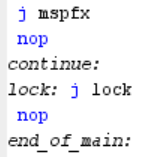
\includegraphics[scale=1]{1.vut} \quad và \quad 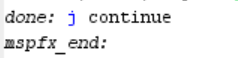
\includegraphics[scale=1]{1.vut2} để tránh vòng lặp vô hạn.
\\\textbf{Giải thích:}
\begin{itemize}
	\item Khởi tạo giá trị:\begin{center}
	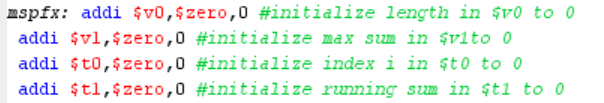
\includegraphics[scale=1]{1.1}
	\end{center}
		Các câu lệnh này thực hiện khởi tạo giá trị cho các biến. \$v0 là độ dài của prefix có tổng lớn nhất. \$v1 là tổng của prefix lớn nhất. \$t0 là giá trị của biến đếm i. \$t1 chứa giá trị tổng của prefix hiện tại.
	\item Vòng lặp:\begin{center}
	 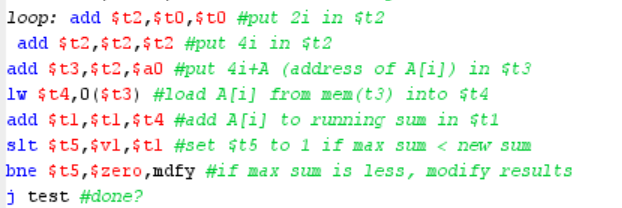
\includegraphics[scale=1]{1.2}
	\end{center}
		Các câu lệnh này là thân của vòng lặp. 4 câu lệnh đầu thực hiện gán giá trị A[i] cho thanh ghi \$t4. Câu lệnh \colorbox{code}{add \$t1,\$t1,\$t4} thực hiện cộng A[i] cho tổng prefix hiện tại. Câu lệnh \colorbox{code}{slt \$t5,\$v1,\$t1} và \colorbox{code}{bne \$t5,\$zero,mdfy} thực hiện rẽ đến nhánh mdfy nếu \textit{max tổng prefix} < \textit{tổng prefix hiện tại}. Nếu không thì \textit{jump} đến nhánh test.
	\item Nhánh mdfy:\begin{center}
	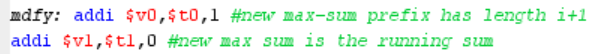
\includegraphics[scale=1]{1.3}
	\end{center}
	Câu lệnh \colorbox{code}{addi \$v0,\$t0,1} thực hiện cập nhật giá trị cho độ dài của max prefix mới. Câu lệnh \colorbox{code}{addi \$v1,\$t1,0} cập nhật giá trị \textit{max tổng prefix} = \textit{tổng prefix hiện tại}.
	\item Nhánh test: \begin{center}
	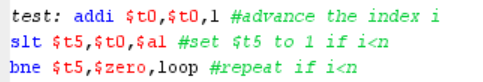
\includegraphics[scale=1]{1.4}
	\end{center}
	3 câu lệnh này thực hiện cập nhật giá trị cho biến đếm i, nếu \textit{i<n} thì quay lại nhãn \textit{loop}. Nếu không thì kết thúc chương trình.
\end{itemize}
\pagebreak
\section*{\begin{huge}
Assignment 2
\end{huge}}
\textbf{Mã nguồn:}
\begin{center}
\begin{lstlisting}
.data
A: .word 7, -2, 5, 1, 5,6,7,3,6,8,8,59,5
Aend: .word 

.text
main: la $a0,A #$a0 = Address(A[0])
 la $a1,Aend
 addi $a1,$a1,-4 #$a1 = Address(A[n-1])
 j sort #sort
after_sort: li $v0, 10 #exit
 syscall
end_main:
#--------------------------------------------------------------
#procedure sort (ascending selection sort using pointer)
#register usage in sort program
#$a0 pointer to the first element in unsorted part
#$a1 pointer to the last element in unsorted part
#$t0 temporary place for value of last element
#$v0 pointer to max element in unsorted part
#$v1 value of max element in unsorted part
#--------------------------------------------------------------
sort: beq $a0,$a1,done #single element list is sorted
 j max #call the max procedure
after_max: lw $t0,0($a1) #load last element into $t0
 sw $t0,0($v0) #copy last element to max location
 sw $v1,0($a1) #copy max value to last element
 addi $a1,$a1,-4 #decrement pointer to last element
 j sort #repeat sort for smaller list
done: j after_sort
#Procedure max
#function: fax the value and address of max element in the list
#$a0 pointer to first element
#$a1 pointer to last element
#------------------------------------------------------------------------
max:
 addi $v0,$a0,0 #init max pointer to first element
 lw $v1,0($v0) #init max value to first value
 addi $t0,$a0,0 #init next pointer to first
loop:
 beq $t0,$a1,ret #if next=last, return
 addi $t0,$t0,4 #advance to next element
 lw $t1,0($t0) #load next element into $t1
 slt $t2,$t1,$v1 #(next)<(max) ?
 bne $t2,$zero,loop #if (next)<(max), repeat
 addi $v0,$t0,0 #next element is new max element
 addi $v1,$t1,0 #next value is new max value
 j loop #change completed; now repeat
ret:
 j after_max
\end{lstlisting}
\end{center}
\textbf{Lưu ý: } 2 mảng A và Aend được khởi tạo liên tiếp nhau, vậy nên địa chỉ của con trỏ Aend cũng nằm ngay sau địa chỉ con trỏ của A[n]. Vậy nếu ta muốn trỏ đến phần tử cuối cùng của mảng A, ta chỉ cần câu lệnh \colorbox{code}{addi \$a1,\$a1,-4} là \$a1 sẽ trỏ đến phần tử A[n].\\
\textbf{Giải thích:}
\begin{itemize}
	\item Bắt đầu chương trình:
		\begin{center}
		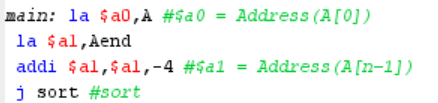
\includegraphics[scale=1]{2.1}
		\end{center}
	Load địa chỉ các mảng vào các thanh ghi. Thanh ghi \$a0 chứa địa chỉ của A[i], thanh ghi \$a1 chứa địa chỉ của A[n]. Sau đó chương trình nhảy đến nhánh \textit{sort}. 
	\item Nhánh \textit{sort}:
		\begin{center}
		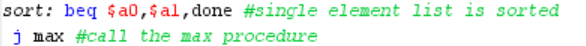
\includegraphics[scale=1]{2.2}
		\end{center}
	Lệnh \colorbox{code}{beq \$a0,\$a1,done} sẽ nhảy đến nhánh done nếu chương trình đã duyệt qua hết tất cả phần tử trong mảng. (Địa chỉ thanh ghi \$a0 = \$a1). Nếu không thì nhảy đến nhánh max.
	\item Nhánh \textit{max} và \textit{loop}:
		\begin{center}
		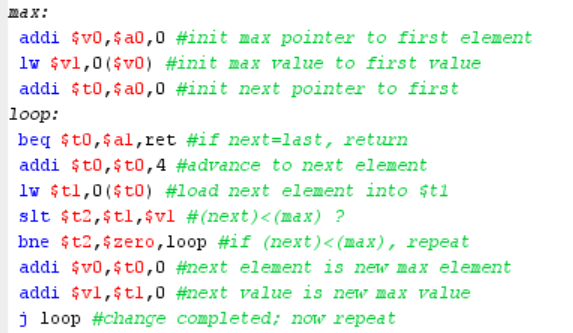
\includegraphics[scale=1]{2.3}
		\end{center}
	\begin{itemize}
		\item Nhánh \textit{max} khởi tạo các giá trị ban đầu: thanh ghi \$v0 chứa địa chỉ của phần tử có giá trị lớn nhất của dãy con chưa được sắp xếp, thanh ghi. \$v1 chứa giá trị của phần tử lớn nhất của dãy con chưa được sắp xếp, thanh ghi \$t0 chứa địa chỉ của phần tử tiếp theo.
	    \item Nhánh \textit{loop}:
	    		\begin{itemize}
	    		\item Câu lệnh \colorbox{code}{beq \$t0,\$a1,ret} thực hiện rẽ đến nhánh \textit{ret} nếu đã duyệt đến phần tử cuối cùng của dãy con chưa được sắp xếp.
	    		\item 2 câu lệnh \colorbox{code}{addi} và \colorbox{code}{lw} thực hiện gán giá trị phần tử tiếp theo cho thanh ghi \$t1. (\textit{Cách duyệt đến phần tử kế tiếp này là khác so với cách duyệt ở Assignment 1}).
	    		\item 2 câu lệnh \colorbox{code}{slt \$t2,\$t1,\$v1} và \colorbox{code}{bne \$t2,\$zero,loop} sẽ thực hiện quay lại nhánh loop này nếu \textit{phần tử hiện tại} $\leq$ \textit{max}.
	    		\item Nếu \textit{phần tử hiện tại} $>$ \textit{max} thì thực hiện câu lệnh \colorbox{code}{addi \$v0,\$t0,0} (gán \textit{phần tử hiện tại} = \textit{phần tử max}) và \colorbox{code}{addi \$v1,\$t1,0}
	    		\end{itemize}
	\end{itemize}
\end{itemize}
\end{document}